\chapter{eBPF}
\section{歴史的背景}
\subsection{Berkeley Packet Filter}
StevenとVan \cite{berkeley-packet-filter}は1993年に,Unix系のOS上でパケットキャプチャを効率的に行うためのアーキテクチャである
Berkeley Packet Filterを提案した.
これ以降,Berkeley Packet Filterを「BPF」と表記する.
BPFが登場する以前のパケットキャプチャでは,カーネル空間で取得したパケットをすべてユーザー空間にコピーしてからフィルタリングしていて,
これが無駄なオーバーヘッドの原因となっていた.
\cite{berkeley-packet-filter}では特殊な32ビットの命令セットを解釈してパケットフィルタリングを行う擬似マシン (BPF pseudo-machine) を提案し,
この擬似マシンをカーネル空間で動作させることでオーバーヘッドを軽減することを目指した.

BPFはLinuxカーネルのv2.1.75にてLinux Socket Filterとして導入され,\texttt{tcpdump}コマンドの高速化に利用された.
既存のシステムとの比較では,BPF は最大で20倍程度高速にパケットキャプチャを行うことができた.

\subsection{eBPF: extended BPF}
BPFはLinux カーネルのv3.18にて大幅に拡張が行われ,extended BPFすなわちeBPFと呼ばれるようになった.
eBPF以前のBPFを明確に区別するためにcBPF (classical BPF) と呼ぶことがある.
拡張された項目は多岐にわたるが,代表的な項目を以下に示す.
\begin{itemize}
  \item BPF命令セットが32ビットから64ビットに書き直され,実行効率が向上した.
  \item eBPF mapというデータ構造が導入され,ユーザ空間とカーネル空間の間でのデータ共有や,eBPFプログラム内のデータ保存またはプログラム間でのデータ共有が可能になった.
  \item eBPFプログラムが安全に実行できることを検証するeBPF verifierが追加された.
\end{itemize}

上述した拡張に加えて,eBPFはその適用範囲を大きく拡大してきた.
ネットワーク分野においては,Linuxネットワークスタック内の様々なレイヤー,例えばトランスポート層 (e.g. TCP/UDP) や
データリンク層 (e.g. ネットワークデバイスドライバ) などを対象に処理を記述することが可能となった.
さらにeBPFはパフォーマンストレーシングやセキュリティ機能の向上にも活用されるようになっている.
これに伴い,「BPF」という用語は元々の「Berkeley Packet Filter」という意味を超えて,独立したフレームワークを指す言葉として
認識されるようになった.

\section{eBPFのアーキテクチャ}
eBPFシステムの概要を\figref{fig:ebpf-overview}に示す.
特殊なC言語で記述されたeBPFプログラムはBPFバイトコードにコンパイルされ,\texttt{bpf}システムコールを通じてカーネルにロードされる.
ロードされたeBPFプログラムはeBPF verifierによって検証され,安全性が確認された後にJITコンパイルされ,カーネル内で実行される.
本研究におけるFugaの実装に関連性の高い要素について詳述する.
\begin{figure}[t]
  \begin{center}
    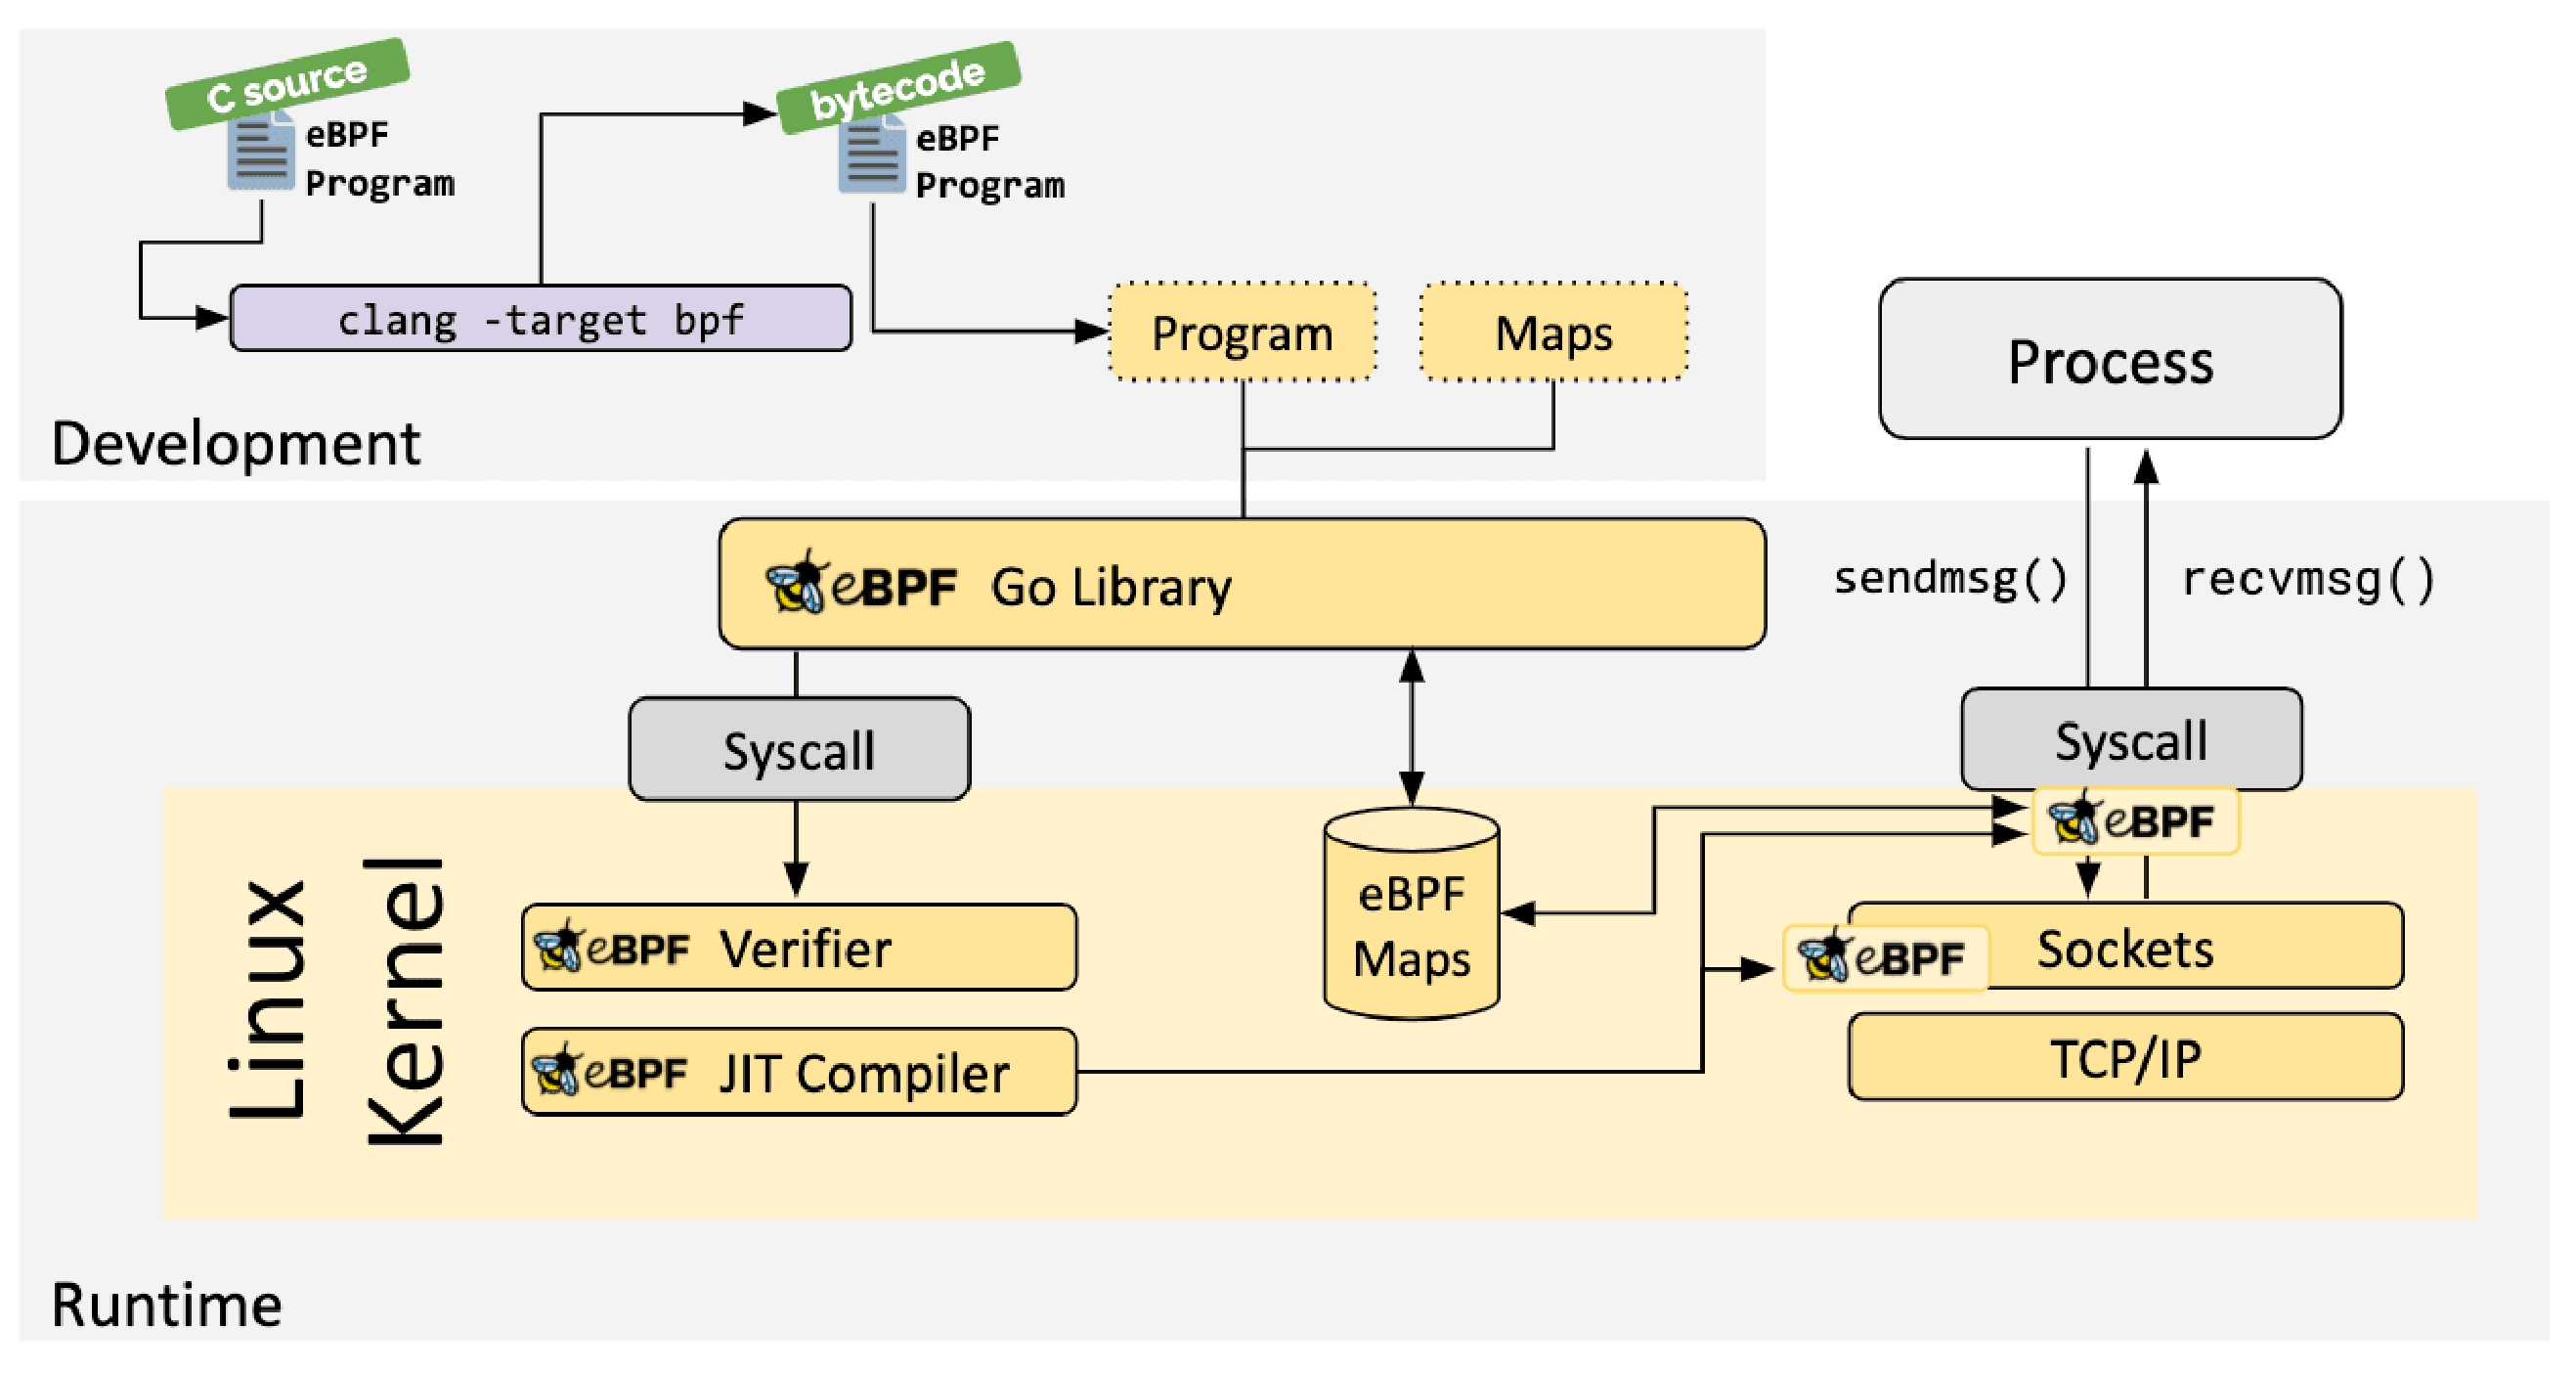
\includegraphics[width=0.8\columnwidth]{doc/img/ebpf-overview.eps}
  \end{center}
  \caption{Overview of eBPF system. \cite{WhatiseB81:online}}
  \label{fig:ebpf-overview}
\end{figure}

\subsection{イベント駆動型アーキテクチャ}
eBPFはイベント駆動型のアーキテクチャを採用している.
すなわち,開発者はカーネル空間またはユーザ空間で発生する特定のイベントをeBPFプログラムでフックし,イベント発生時にプログラムが実行される
ようにカーネルの動作を拡張することができる.
eBPFプログラムでイベントをフックすることを「eBPFプログラムをアタッチする」と表現するが,
プログラムのロードおよびアンロード,アタッチおよびデタッチは動的に行えるように実装されている.

% 例えばXDPはネットワークインタフェースの受信パケット処理にeBPFプログラムをアタッチするためのprogram typeである.
% eBPFにはprogram typeという概念があり,これはeBPFプログラムがどのようなイベントにフックされるかを示す.
eBPFにはフックポイントという概念があり,eBPFプログラムが特定のイベントに応じて動作するために接続されるカーネルやユーザスペースの機能的なエントリポイントを指す.
本研究におけるFugaの実装では以下のフックポイントを利用している.
\begin{itemize}
  \item \textbf{uprobe}:ユーザ空間プログラムが実行する関数のエントリ
  \item \textbf{fentry/fexit}:カーネル関数のエントリ/終了
\end{itemize}
こられのフックポイントではフックする先の関数をeBPFプログラム内に記述する.指定した関数が呼び出されると,
その関数のエントリや終了時にeBPFプログラムが実行される.

\subsection{eBPF Verifier}
eBPF verifierはバイトコードに変換されたeBPFプログラムを入力として受け付けて,
そのプログラムがカーネル上で安全に実行できることを検証するプログラムである.
verifierの検査項目としては,
プログラムのメモリアクセス違反,正常終了性 (無限ループする可能性があるかどうか),
スタックサイズや命令数の上限の超過などが挙げられる
\footnote{命令の上限数は,cBPFにおいて4096,eBPFにおいて100万である.}.
eBPFプログラムはverifierによる安全性の検証を通過しない限り実行されないという点において,
eBPFは一定レベルの安全性が保障されている.

\subsection{eBPF Map}
eBPF map (以下,map) はeBPFプログラムおよびユーザ空間の両方からアクセス可能なデータ構造である.
mapは複数のeBPFプログラム間でデータを共有したり,eBPFプログラムとユーザ空間プログラム間でデータを
授受したりするために利用される.
典型的なユースケースは以下の通り\cite{learning-eBPF}.
\begin{itemize}
  \item ユーザ空間にて設定情報を書き込み,eBPFプログラムがそれを取得する.
  \item あるeBPFプログラムがステートを保存し,後に同一プログラムまたは別のプログラムが参照する.
  \item eBPFプログラムがメトリクスをmapに書き込み,ユーザ空間プログラムがmapから取得して可視化を行う.
\end{itemize}
配列やキューなど複数のデータ構造がmapとして提供されているが,本研究においては
\textbf{ハッシュテーブル}と\textbf{リングバッファ}を利用している.
eBPFにおけるリングバッファは,eBPFプログラムからユーザ空間への高頻度なデータ転送に適している.
